\documentclass[11pt]{scrartcl}

\usepackage[top=1in, bottom=2cm, left=1in, right=1in]{geometry}
\usepackage{graphicx}
\usepackage{amsmath}
\usepackage{subfig}

\begin{document}

\title{Project 1 STAT5376}
\subtitle{Bayesian Analysis of Noisy Images}
\author{Li Sun}
\date{\today}
\maketitle

\noindent
1. Goal: Given observed noisy images, our goal is to perform a Bayesian analysis of this data. We will assume a prior probability model and an observation model to obtain a posterior density, and will generate samples from the posterior.

\bigskip

\noindent
2. Models\\
(a)Prior Model: \\
$$f(I_{i,j}|\text{all other pixels})=f(I_{i,j}|I_{i,j-1},I_{i-1,j},I_{i+1,j},I_{i,j+1})=N(m,\sigma^2_1)$$
All conditional density of a pixel of this m by n Markov Random field only depends on 4 adjacent pixels, 3 for edge pixels and 2 for corner pixels. The m is mean of all neighbors\\

\bigskip

(b)Observation Model:
$$D=I+W$$
where each element of $W$ is an independent normal random variable with mean $0$ and variance $\sigma^2_2$. This specifies the conditional likelihood function 
$$f(D|I) \sim N(D_{i,j}, \sigma^2_2)$$

\bigskip

(c)So we can have our conditional posterior density
$$f(I|D)=f(D|I)f(I)$$
Given the structure of $f(I)$ and independence of elements of W, the full conditional of this posterior density can be written as:
$$f(I_{i,j}|D, \text{all other pexels}) \propto N(m,\sigma^2_1)N(D_{i,j}, \sigma^2_2)$$

\bigskip

3.To generate sample from full posterior, which is not available, we can use Gibbs Sampler to sample from full conditionals sequentially. However, the full conditional density is not a common density which we could sample easily. So we will use MH method for each pixel.\\
To sample from full conditionals using MH, we chose 
$$q(x) \sim N(m,\sigma^2_1)$$
as our proposal for convenience of calculation. So the acceptance rate is calculated as:
$$
\begin{array}{lcl}
\rho(x, y) &=& min\left\{1,\frac{f(y)q(x)}{f(x)q(y)}\right\}\\
&=& min\left\{1,exp(\frac{1}{2\sigma^2_2}((x-D_{i,j})^2-(y-D_{i,j})^2))\right\}
\end{array}
$$
To make our simulation more efficient, we better make our MH algorithm more efficient. So we should do some tests on this MH algorithm. We tested how it perform under several different $\sigma_2(10,20,100)$, $m$, $D_{i,j}()$ and different iterations of MH process.\\
Our aim is to sample from our target density, so we want to make sure the Markov chain produced by our MH algorithm converges before we take values. As a simple way of checking this, we check the convergence of the mean of our target posterior density
$$\frac{1}{Z}N(m,\sigma_1)N(D_{i,j},\sigma^2_2)$$
The 'true mean' of this density is determined by Monte Carlo integration and the difference between this 'true mean' and our converged mean from our MH Markov chain was calculated based on changing factors of $\sigma_2(10,20,100)$, $m$, $D_{i,j}()$ and two different iteration numbers(100 and 500). The result is as followed:\\
\begin{figure}
\centering
\subfloat[$\sigma_1$=10 with 100 MH iterations]{
  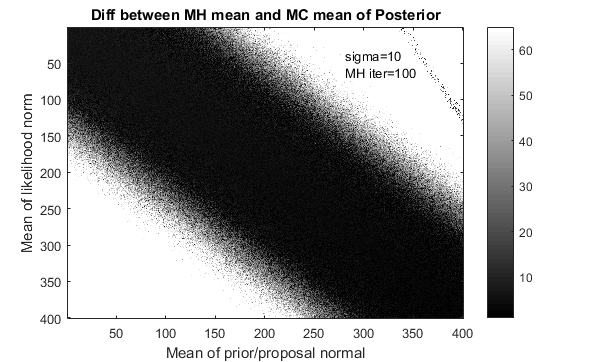
\includegraphics[width=65mm]{validateingMH100s10.png}
}
\subfloat[$\sigma_1$=10 with 500 MH iterations]{
  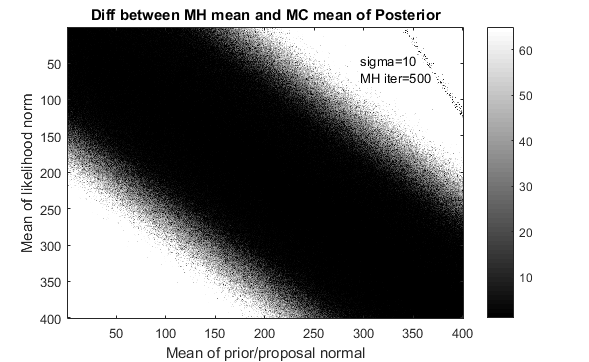
\includegraphics[width=65mm]{validateingMH500s10.png}
}
\hspace{0mm}
\subfloat[$\sigma_1$=20 with 100 MH iterations]{
  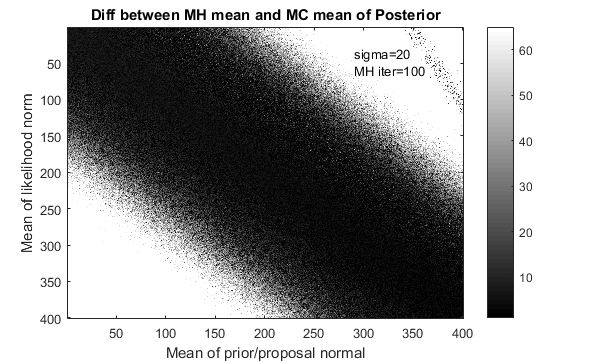
\includegraphics[width=65mm]{validateingMH100s20.png}
}
\subfloat[$\sigma_1$=20 with 500 MH iterations]{
  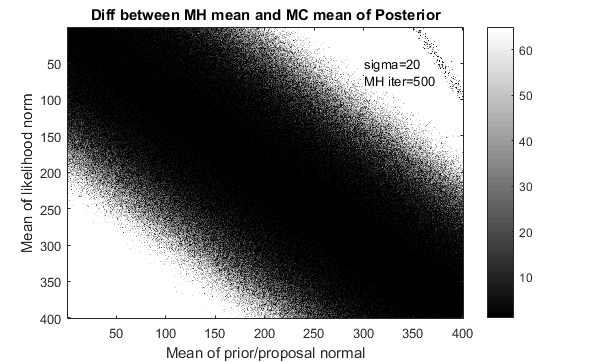
\includegraphics[width=65mm]{validateingMH500s20.png}
}
\hspace{0mm}
\subfloat[$\sigma_1$=100 with 100 MH iterations]{  
  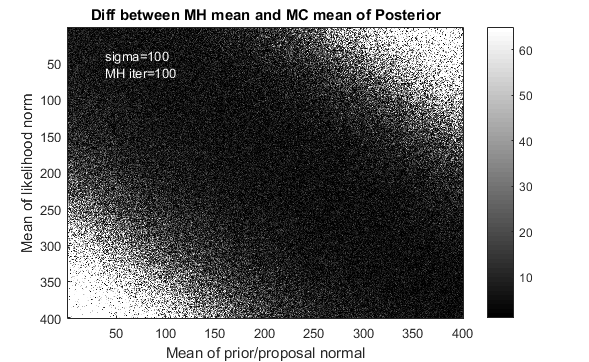
\includegraphics[width=65mm]{validateingMH100s100.png}
}
\subfloat[$\sigma_1$=100 with 500 MH iterations]{
  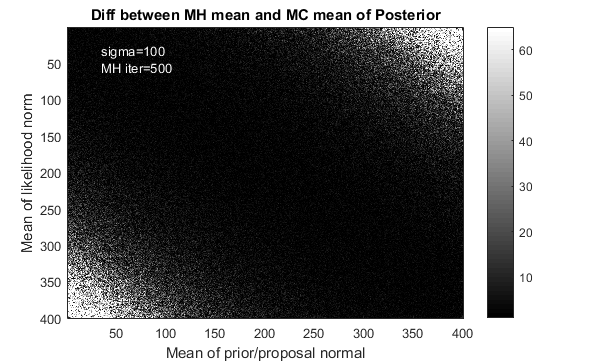
\includegraphics[width=65mm]{validateingMH500s100.png}
}
\caption{caption}
\end{figure}

Conclusion is that, our MH algorithm works reasonably well when difference between $m$ and $D_{i,j}$ are close(the difference are smaller than 100) in all cases. 100 iteration seem to perform well enough if the two means are close enough. And we know that
$$D=I+W$$
and the standard deviation of W is 30. So the possibility that difference between D and I are larger than 100 is slime. So we will use this MH algorithm and take 100th number as our sampled value each time.\\

\bigskip
4. Choose the initial value. In order for Gibbs sampling converge quickly, I will set my best guess, which is the noisy image as initial values.\\

\bigskip

5. Results.\\
(a)When $\sigma_1=10$:\\
I start using 1000 iteration for Gibbs sampling. And the evolution of D1 when $\sigma_1=10$ is as followed\\
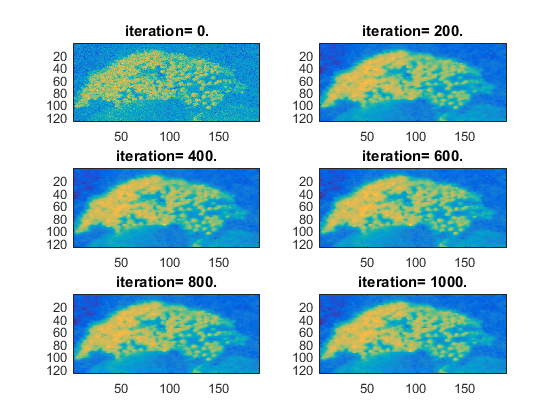
\includegraphics[scale=1]{D1_1000.png}\\
What we observed is much more smooth picture after sampling. However, As you can see that after 200 iteration, the change of the picture are undetectable, which means it converged. So to see the evolution of pictures, we use less iterations instead (20). \\
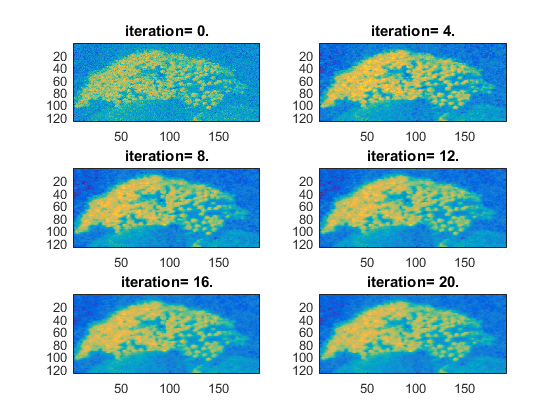
\includegraphics[scale=1]{D1_20.png}\\
I am surprised how quickly this chain converge, or it is because the difference later is just undetectable to our eyes?\\
(b)When $\sigma_1=20$:\\
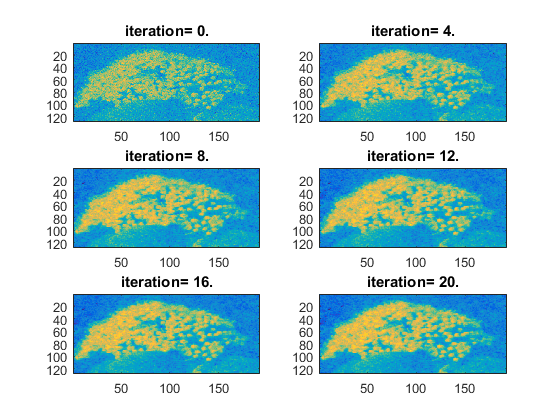
\includegraphics[scale=1]{D1_20_20.png}\\
It looks like images converge slower.\\
(c)When $\sigma_1=100$:\\
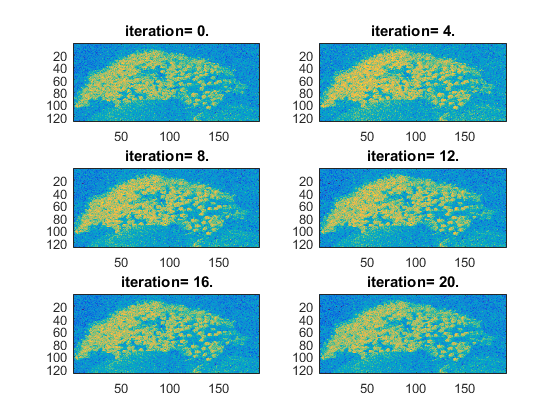
\includegraphics[scale=1]{D1_100_20.png}\\
It converges much worse. So for smaller $\sigma1$, we have faster convergence. This applys to all other picture, so I pick only $\sigma_1=10$ and use 20 iteration to see the evolution of pictures. The results see later pages.\\
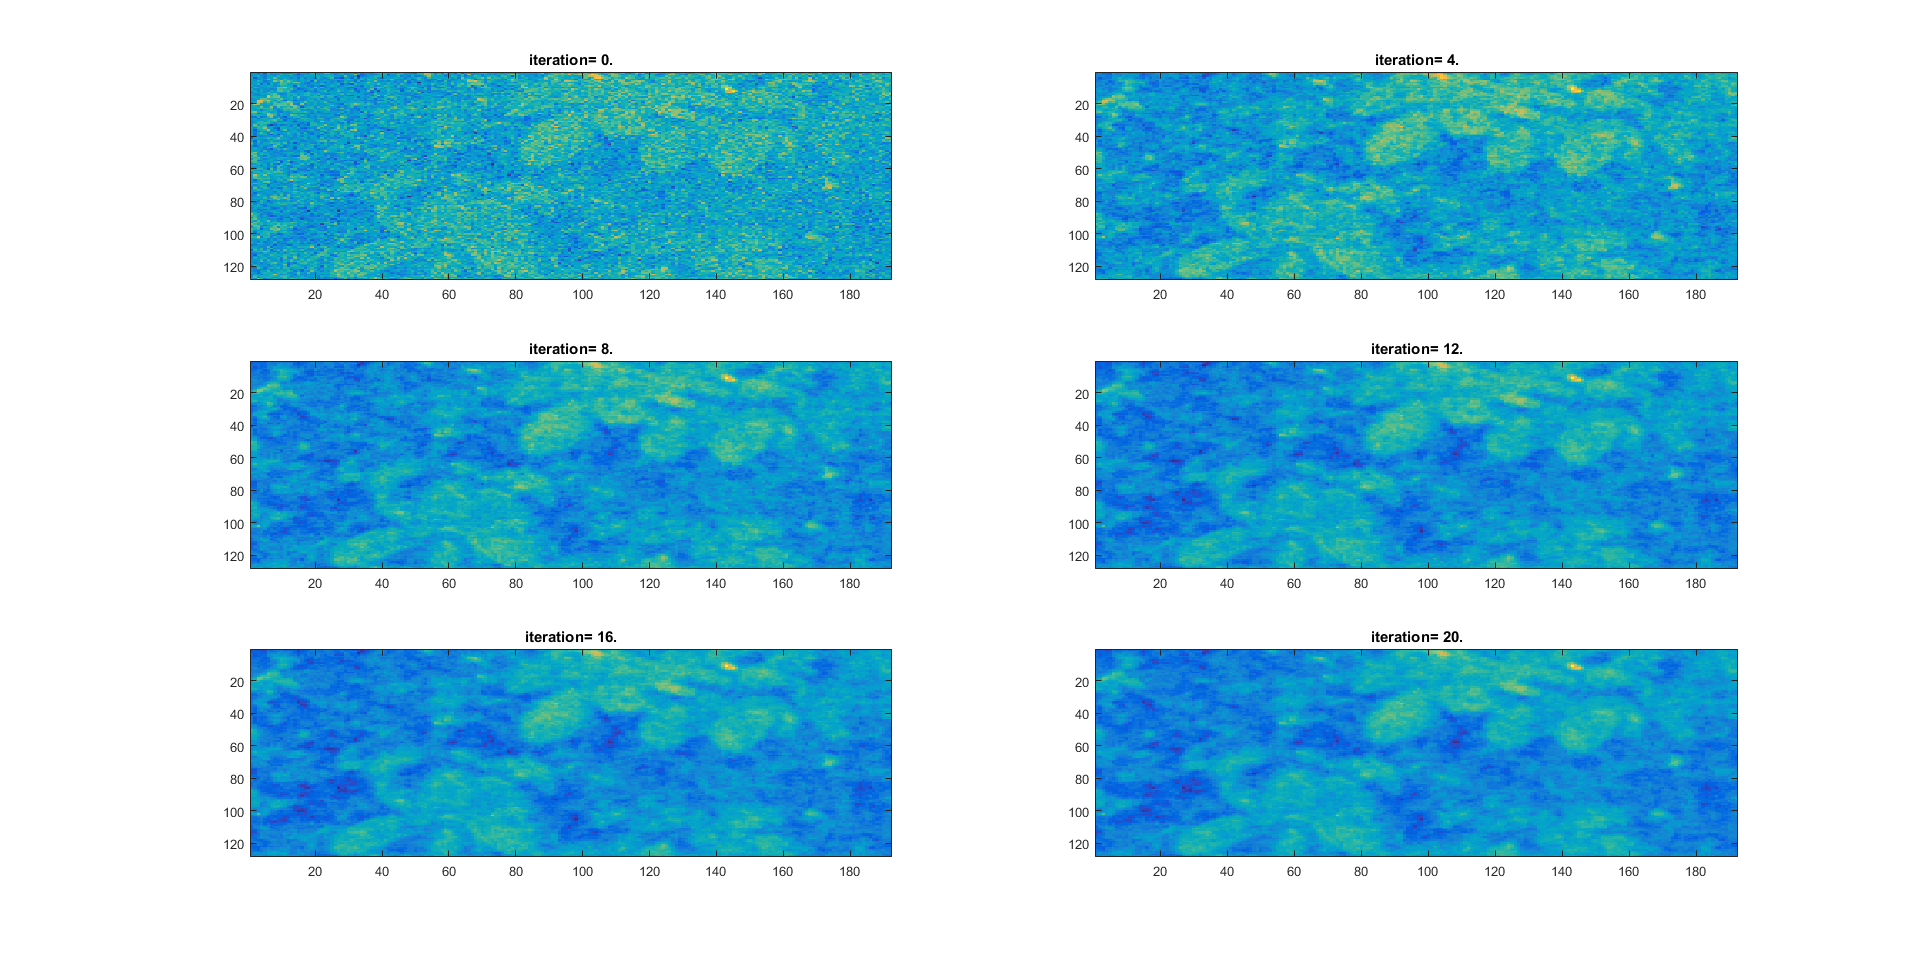
\includegraphics[width=160mm,height=160mm]{D2_10_20.png}\\
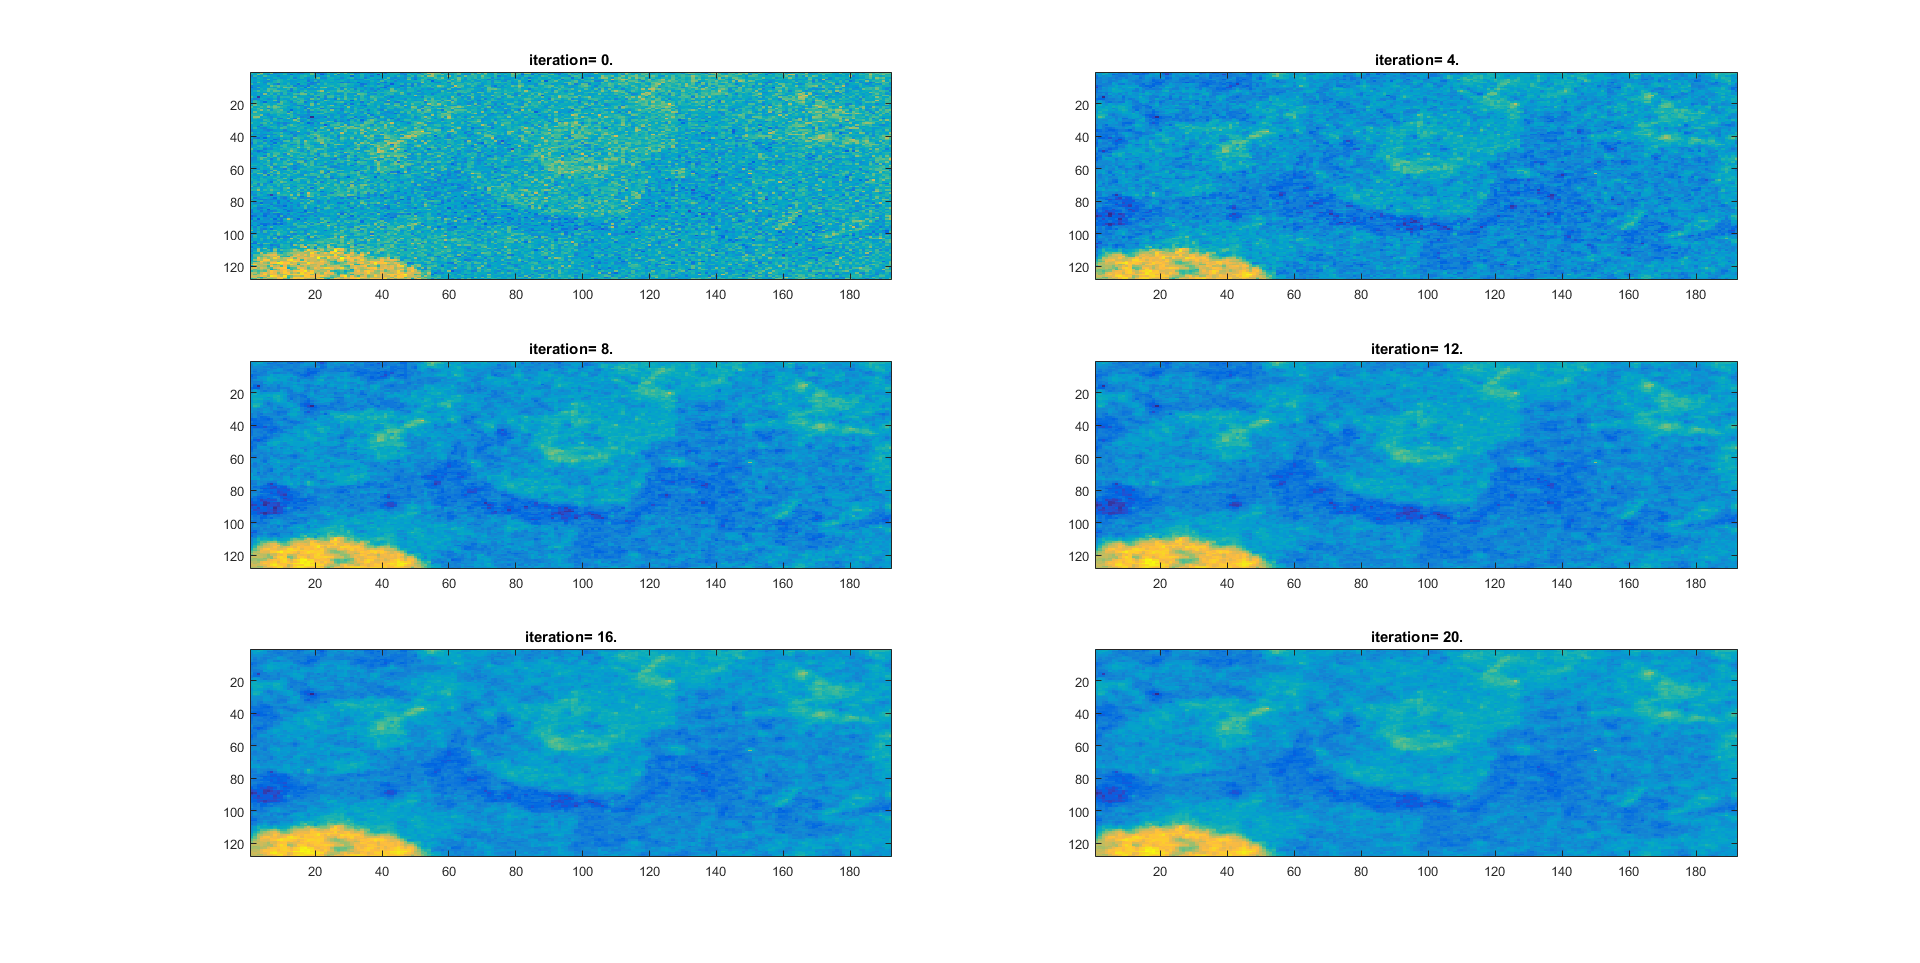
\includegraphics[width=160mm,height=160mm]{D3_10_20.png}\\
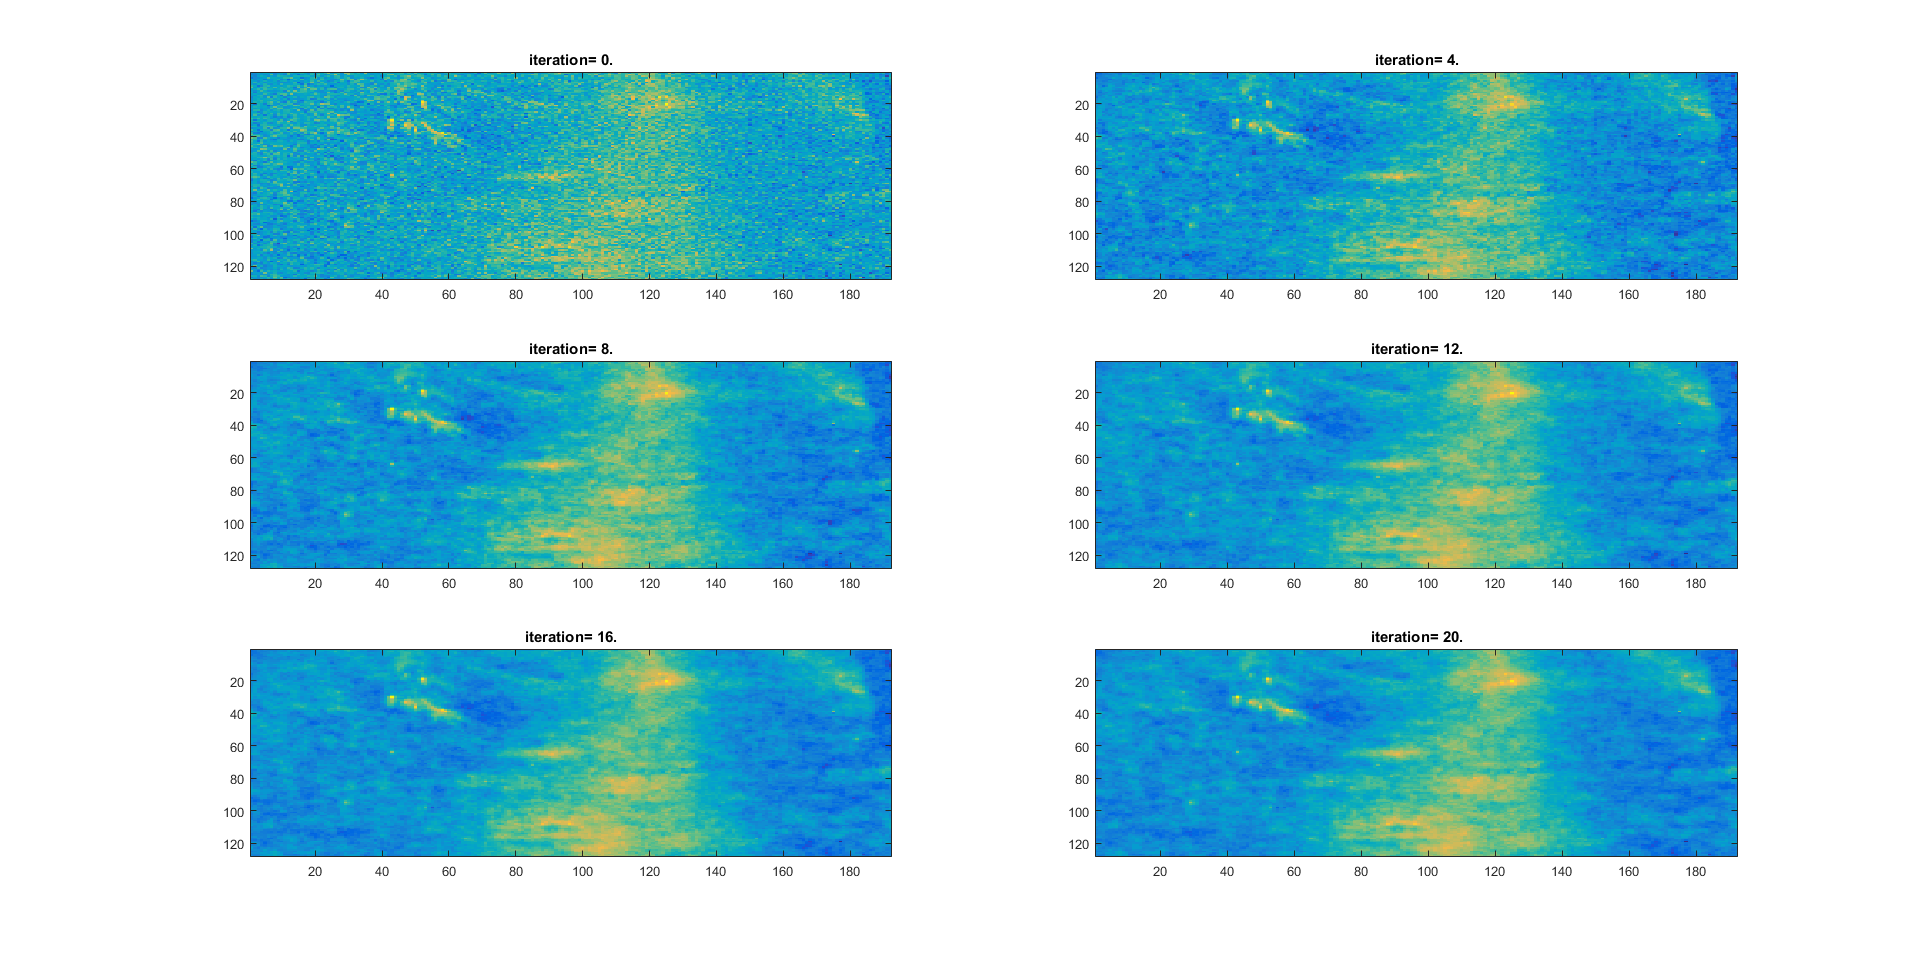
\includegraphics[width=160mm,height=160mm]{D4_10_20.png}\\
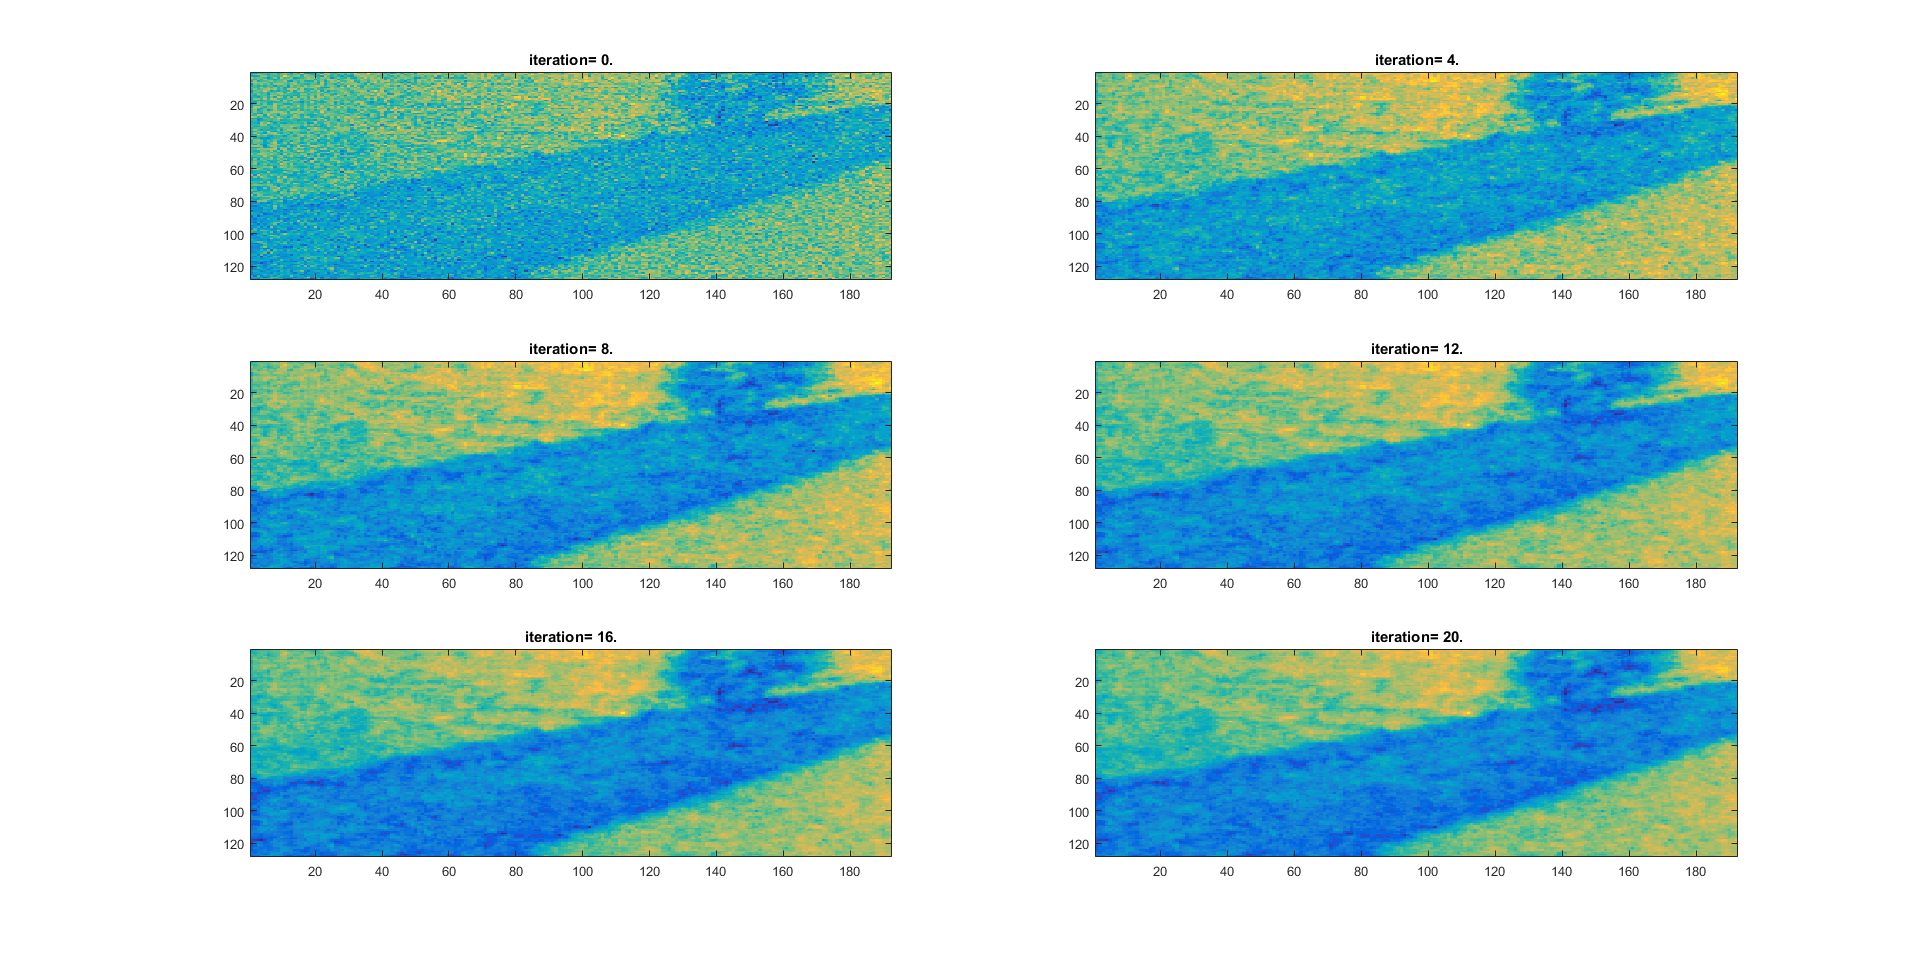
\includegraphics[width=160mm,height=160mm]{D5_10_20.png}\\
\bigskip

Above all, this MCMC program simulates the posterior density of our bayesian model about our pictures. And after iteration of convergence, the noisy figure got smoothed reasonably well under small variance. \\

\bigskip

All code please see https://github.com/rikku1983/STAT5376\\
\bigskip

Thanks!


\end{document}